\documentclass{beamer}
\usetheme[faculty=ped,basePath=../fibeamer,logo=../fibeamer/logo/mu/Logo-UC-3.png]{fibeamer}
\graphicspath{{../resources/}}

\usepackage{algorithm}
\usepackage{algpseudocode}

\usetheme[faculty=ped]{fibeamer}
\usepackage[utf8]{inputenc}
\usepackage[
  main=english,
  czech, slovak
]{babel}
\title{Ordenamiento}
\subtitle{Semestre II-2026}
\author{Profesora: Andreina Cota Vidaurre}

\usepackage{ragged2e}
\usepackage{booktabs}
\usepackage{tabularx}
\usepackage{tikz}
\usetikzlibrary{calc, shapes, backgrounds}
\usetikzlibrary{positioning, arrows.meta, shadows.blur, shapes.geometric}
\usepackage{amsmath, amssymb}
\usepackage{url}
\usepackage{listings}
\usepackage{graphicx}
\usepackage{amsmath}
\usepackage[T1]{fontenc}
\usepackage{xcolor}
\usepackage{minted}

\lstdefinelanguage{PseudocodigoES}{
    morekeywords={INICIO,FIN,PARA,HACER,SI,ENTONCES,FIN_SI,FIN_PARA,IMPRIMIR},
    sensitive=true,
    morecomment=[l]{//},
    morestring=[b]"
}

\lstdefinelanguage{PseudocodeEN}{
    morekeywords={BEGIN,END,FOR,DO,IF,THEN,END_IF,END_FOR,PRINT},
    sensitive=true,
    morecomment=[l]{//},
    morestring=[b]"
}

\lstset{
    basicstyle=\ttfamily\small,
    keywordstyle=\bfseries,
    columns=fullflexible,
    keepspaces=true,
    showstringspaces=false,
    frame=single,
    xleftmargin=0em,
    framexleftmargin=0em,
    framesep=2pt,
    gobble=4,
    resetmargins=true,
    aboveskip=0pt,
    belowskip=0pt
}

\lstdefinestyle{pythonstyle}{
    language=Python,
    basicstyle=\ttfamily\small,
    keywordstyle=\bfseries,
    commentstyle=\itshape,
    stringstyle=\ttfamily,
    showstringspaces=false,
    columns=fullflexible,
    keepspaces=true,
    frame=single,
    breaklines=true,
    xleftmargin=0em,
    framexleftmargin=0em,
    framesep=2pt,
    aboveskip=0pt,
    belowskip=0pt,
    gobble=4,
    resetmargins=true,
    emph={print,input,int,float,str,bool,len,range,sorted,sort,reverse,key},
    emphstyle=\bfseries
}

\lstset{style=pythonstyle}

\tikzstyle{iniciofin} = [
    ellipse,
    minimum width=2.5cm,
    minimum height=1cm,
    text centered,
    draw=black,
    fill=blue!25
]

\tikzstyle{proceso} = [
    rectangle,
    rounded corners,
    minimum width=3cm,
    minimum height=1cm,
    text centered,
    draw=black,
    fill=cyan!20
]

\tikzstyle{decision} = [
    diamond,
    aspect=2,
    text centered,
    draw=black,
    fill=yellow!35
]

\tikzstyle{flecha} = [
    thick,
    ->,
    >=Stealth
]

\frenchspacing
\begin{document}
  \shorthandoff{-}
  \frame[c]{\maketitle}

    %------------------------------------------------------------------
    \begin{frame}{Contenido}
        \begin{itemize}
            \item Introducción
            \item Ordenamiento con \mintinline{python}{sort()}
            \begin{itemize}
                \item Orden creciente y decreciente
                \item Criterio propio con \mintinline{python}{key=}
                \item Múltiples criterios
            \end{itemize}
            \item Algoritmos de ordenamiento
            \begin{itemize}
                \item Algoritmo de selección
                \item Existencia de algoritmos más eficientes
            \end{itemize}
            \item Ejercicios
            \item Resumen
        \end{itemize}
    \end{frame}

    %------------------------------------------------------------------
    \begin{frame}{Introducción}
        \textcolor{blue}{\textbf{¿Por qué es importante ordenar datos?}}
    \end{frame}

    \begin{frame}[fragile, t]{Introducción}
        \textcolor{blue}{\textbf{¿Cómo podemos organizar una lista de estudiantes según sus calificaciones?}}
        
        Por ejemplo, si tenemos la siguiente lista de notas:

        \begin{minted}[xleftmargin=-2cm, frame=leftline, fontsize=\small]{python}
            notas = [5.0, 3.8, 6.2, 4.1, 2.9]
        \end{minted}
    \end{frame}

    \begin{frame}[fragile, t]{Introducción}
        \textcolor{blue}{\textbf{¿Cómo podemos organizar una lista de estudiantes según sus calificaciones?}}
        
        Por ejemplo, si tenemos la siguiente lista de notas:

        \begin{minted}[xleftmargin=-2cm, frame=leftline, fontsize=\small]{python}
            notas = [5.0, 3.8, 6.2, 4.1, 2.9]
        \end{minted}

        Queremos conocer:
        \begin{itemize}
            \item ¿Cuáles son las mejores calificaciones?
            \item ¿Cuál es la calificación más baja?
            \item ¿Cómo podemos ordenar las notas de menor a mayor?
        \end{itemize}
    \end{frame}

    \begin{frame}[fragile, t]{Introducción: Ordenamiento}
        \begin{itemize}
            \item \textbf{Ordenamiento} es el proceso de reorganizar los elementos de una colección 
            según un criterio establecido.
            \item Los criterios pueden ser numéricos, alfabéticos, de duración, etc.
            \item El criterio determina cómo se comparan y organizan los elementos.
        \end{itemize}
        
        % IMAGEN SUGERIDA:
        % En Python, las listas incluyen el método \mintinline{python}{sort()} para hacerlo.
    \end{frame}

    %------------------------------------------------------------------
    \begin{frame}[fragile, t]{Ordenamiento en Python: \mintinline{python}{sort()}}
        \mintinline{python}{sort()} reorganiza los elementos de una lista en forma ascendente,
        siempre que sus elementos sean comparables entre sí.

        \pause

        \mintinline{python}{sort()} ordena la lista \textbf{in-place}:
        modifica la lista original y no retorna una nueva.

        \pause

        \mintinline{python}{sort(reverse=True)} ordena la lista de forma decreciente.
    \end{frame}

    \begin{frame}[fragile, t]{Ordenamiento en Python: \mintinline{python}{sort()}}
        \begin{minted}[xleftmargin=-2cm, frame=leftline, fontsize=\small]{python}
            notas = [5.0, 3.8, 6.2, 4.1, 2.9]
            notas.sort()
            print(notas)
            # [2.9, 3.8, 4.1, 5.0, 6.2]
        \end{minted}

        \vspace{0.3em}
        \begin{minted}[xleftmargin=-2cm, frame=leftline, fontsize=\small]{python}
            ciudades = ["Valparaíso", "Santiago", "Concepción", "Arica"]
            ciudades.sort()
            print(ciudades)
            # ['Arica', 'Concepción', 'Santiago', 'Valparaíso']
        \end{minted}
    \end{frame}

    %------------------------------------------------------------------
    \begin{frame}[fragile, t]{Ordenamiento en Python: \mintinline{python}{sort(reverse=True)}}
        \begin{minted}[xleftmargin=-2cm, frame=leftline, fontsize=\small]{python}
            puntajes = [120, 95, 200, 150]
            puntajes.sort(reverse=True)
            print(puntajes)
            # [200, 150, 120, 95]
        \end{minted}

        \vspace{0.3em}
        \begin{minted}[xleftmargin=-2cm, frame=leftline, fontsize=\small]{python}
            temperaturas = [18.5, 12.0, 22.3, 9.8, 15.1]
            temperaturas.sort()
            print(temperaturas[0], temperaturas[-1])

            temperaturas.sort(reverse=True)
            print(temperaturas[0])
        \end{minted}
    \end{frame}

    %------------------------------------------------------------------
    \begin{frame}[fragile, t]{Actividad: Ordenamiento}
        Una competencia de videojuegos registra los siguientes puntajes:

        \begin{minted}[xleftmargin=-2cm, frame=leftline, fontsize=\small]{python}
            puntajes = [250, 470, 180, 390, 520, 310]
        \end{minted}
        
        Completa el programa para mostrar:

        \begin{itemize}
            \item Los puntajes ordenados de menor a mayor.
            \item Los puntajes ordenados de mayor a menor.
            \item Los tres mejores puntajes.
        \end{itemize}
    \end{frame}

    \begin{frame}[fragile, t]{Actividad: Ordenamiento}
        \begin{minted}[xleftmargin=-2cm, frame=leftline, fontsize=\small]{python}
            puntajes = [250, 470, 180, 390, 520, 310]

            # Ordenar de menor a mayor
            puntajes.________()
            
            print(puntajes)
            
            # Ordenar de mayor a menor
            puntajes.________(________)
            
            print(puntajes)
            
            # Mostrar los tres mejores puntajes
            print(________)
        \end{minted}
    \end{frame}

    %------------------------------------------------------------------
    \begin{frame}[fragile, t]{Ordenamiento con criterio propio: \mintinline{python}{key=}}

        \textcolor{blue}{\textbf{¿Cómo podemos ordenar las canciones según su duración?}}

        \begin{minted}[xleftmargin=-2cm, frame=leftline, fontsize=\small]{python}
            canciones = [
                ["Shakira", "Waka Waka", 3.4],
                ["Ed Sheeran", "Perfect", 4.2],
                ["Coldplay", "Yellow", 4.1],
                ["Adele", "Hello", 4.9]
            ]
        \end{minted}
    \end{frame}

    \begin{frame}[fragile, t]{Ordenamiento con criterio propio: \mintinline{python}{key=}}
        \begin{itemize}
            \item El método \mintinline{python}{sort()} sin argumentos compara las listas internas 
            lexicográficamente, comenzando por su primer elemento.
            \item Para ordenar por un criterio derivado, usamos \mintinline{python}{key=}.
            \item El parámetro no permite ordenar por criterio propio.
            \item \mintinline{python}{key=} recibe una función que obtiene el valor utilizado 
            para ordenar cada elemento.
        \end{itemize}

        \vspace{0.5em}
        \begin{minted}[xleftmargin=-2cm, frame=leftline, fontsize=\small]{python}
            lista.sort(key=funcion)
        \end{minted}
    \end{frame}

    \begin{frame}[fragile, t]{Ordenamiento con criterio propio: \mintinline{python}{key=}}
        \begin{minted}[xleftmargin=-2cm, frame=leftline, fontsize=\small]{python}
            canciones = [
                ["Shakira", "Waka Waka", 3.4],
                ["Ed Sheeran", "Perfect", 4.2],
                ["Coldplay", "Yellow", 4.1],
                ["Adele", "Hello", 4.9]
            ]

            # Ordenar por duración
            def obtener_duracion(cancion):
                return cancion[2]
            
            canciones.sort(key=obtener_duracion)
            print(canciones)
            # [["Shakira", "Waka Waka", 3.4], ["Coldplay", "Yellow", 4.1], 
            # ["Ed Sheeran", "Perfect", 4.2], ["Adele", "Hello", 4.9]]
        \end{minted}
    \end{frame}

    \begin{frame}[fragile, t]{Ordenamiento con criterio propio: \mintinline{python}{key=}}
        \begin{minted}[xleftmargin=-2cm, frame=leftline, fontsize=\small]{python}
            def obtener_duracion(cancion):
                return cancion[2]
            
            canciones.sort(key=obtener_duracion)
        \end{minted}

        Ordenamiento con \mintinline{python}{lambda} permite crear una función anónima mediante una expresión.

        \begin{minted}[xleftmargin=-2cm, frame=leftline, fontsize=\small]{python}
            lambda parametro: expresion
        \end{minted}

        Ejemplo:
        \begin{minted}[xleftmargin=-2cm, frame=leftline, fontsize=\small]{python}
            canciones.sort(key=lambda x: x[2])
            print(canciones)
            # [["Shakira", "Waka Waka", 3.4], ["Coldplay", "Yellow", 4.1], 
            #["Ed Sheeran", "Perfect", 4.2], ["Adele", "Hello", 4.9]]
        \end{minted}
    \end{frame}

    \begin{frame}[fragile, t]{Ordenamiento de objetos}
        \begin{minted}[xleftmargin=-2cm, frame=leftline, fontsize=\small]{python}
            class Cancion:
                def __init__(self, titulo, duracion):
                    self.titulo = titulo
                    self.duracion = duracion
                def __repr__(self):
                    return self.titulo
            canciones = [
                Cancion("Gracias a la vida", 273),
                Cancion("Tren al sur", 328),
                Cancion("Yellow", 266)
            ]
            def por_duracion(cancion):
                return cancion.duracion
            canciones.sort(key=por_duracion)
            print(canciones) # ["Yellow", "Gracias a la vida", "Tren al sur"]
        \end{minted}
    \end{frame}

    \begin{frame}[fragile, t]{Ordenamiento de objetos}
        \begin{minted}[xleftmargin=-2cm, frame=leftline, fontsize=\small]{python}
            class Producto:
                def __init__(self, nombre, precio):
                    self.nombre = nombre
                    self.precio = precio

            productos = [
                Producto("Audifonos", 120),
                Producto("Teclado", 85),
                Producto("Mouse", 45)
            ]
            productos.sort(key=lambda producto: producto.precio)
            for producto in productos:
                print(producto.nombre, producto.precio) 
        \end{minted}
    \end{frame}

    \begin{frame}[fragile, t]{Ordenamiento de objetos}
        Una tienda tiene una lista de productos con sus respectivos precios.

        Se necesita:
        \begin{enumerate}
            \item Mostrar los productos desde el más barato hasta el más caro.
            \item Ordenarlos desde el más caro hasta el más barato.
            \item Ordenarlos alfabéticamente por nombre.
        \end{enumerate}
    \end{frame}

    \begin{frame}[fragile, t]{Ordenar strings por longitud}
        \begin{minted}[xleftmargin=-2cm, frame=leftline, fontsize=\small]{python}
            palabras = ["sol", "programación", "casa", "universidad"]
            palabras.sort(key=len)
            print(palabras)
            # ['sol', 'casa', 'universidad', 'programación']
        \end{minted}

        \vspace{0.3em}
        Con una función propia:
        \begin{minted}[xleftmargin=-2cm, frame=leftline, fontsize=\small]{python}
            def longitud(texto):
                return len(texto)

            palabras.sort(key=longitud)
        \end{minted}
    \end{frame}

    %------------------------------------------------------------------
    \begin{frame}[fragile, t]{Ordenamiento por múltiples criterios}
        
        \begin{itemize}
            \item Se pueden combinar criterios en una \mintinline{python}{tupla}.
            \item Python compara primero el primer valor; si empatan, el segundo; y así sucesivamente.
            \item La tupla define la prioridad de los criterios.
        \end{itemize}

        \begin{minted}[xleftmargin=-2cm, frame=leftline, fontsize=\small]{python}
            lista.sort(key=lambda elemento: (criterio1, criterio2, ...))
        \end{minted}
    \end{frame}

    \begin{frame}[fragile, t]{Ordenamiento por múltiples criterios}
        \begin{minted}[xleftmargin=-2cm, frame=leftline, fontsize=\scriptsize]{python}
            canciones = [
                ["Violeta Parra", "Gracias a la vida", 273],
                ["Los Prisioneros", "Tren al sur", 328],
                ["Maroon 5", "Girls like you", 273],
                ["Coldplay", "Yellow", 266]
            ]
            canciones.sort(key=lambda c: (c[2], c[1]))
            print(canciones)
            # [["Violeta Parra", "Gracias a la vida", 273], ["Maroon 5", "Girls like you", 273], 
            # ["Los Prisioneros", "Tren al sur", 328], ["Coldplay", "Yellow", 266]]
        \end{minted}

        \begin{minted}[xleftmargin=-2cm, frame=leftline, fontsize=\scriptsize]{python}
            canciones = [
                Cancion("Gracias a la vida", 273),
                Cancion("Tren al sur", 328),
                Cancion("Girls like you", 273),
                Cancion("Yellow", 266)
            ]
            canciones.sort(key=lambda c: (c.duracion, c.titulo))
            print(canciones)
            # [Yellow, Girls like you, Gracias a la vida, Tren al sur]
        \end{minted}
    \end{frame}

    \begin{frame}[fragile, t]{Ordenamiento por múltiples criterios}
        \begin{minted}[xleftmargin=-2cm, frame=leftline, fontsize=\small]{python}
            jugadores = [
                ["Ana", 90, 45],
                ["Pedro", 85, 38],
                ["Carla", 90, 40],
                ["Luis", 85, 42]
            ]
            jugadores.sort(key=lambda jugador: (-jugador[1], jugador[2]))
            print(jugadores)
            # [["Carla", 90, 40], ["Ana", 90, 45], ["Luis", 85, 42], 
            # ["Pedro", 85, 38]]
        \end{minted}
        \begin{itemize}
            \item \mintinline{python}{(-jugador[1])}: mayor puntaje primero.
            \item \mintinline{python}{(jugador[2])}: menor tiempo de juego primero.
            \item El signo negativo es una técnica aplicable a valores \textbf{numéricos} para invertir el orden.
        \end{itemize}
    \end{frame}

    \begin{frame}[fragile, t]{Ejercicio}
        Una competencia de fútbol tiene los siguientes resultados:
        \begin{minted}[xleftmargin=-2cm, frame=leftline, fontsize=\small]{python}
            resultados = [
                ["Equipo A", 12, 5],
                ["Equipo B", 15, 7],
                ["Equipo C", 12, 3],
                ["Equipo D", 15, 4]
            ]
        \end{minted}
        Cada equipo tiene: \mintinline{python}{[nombre, puntos, penalizaciones]}

        La clasificación debe seguir las siguientes reglas:
        \begin{enumerate}
            \item Mayor cantidad de puntos.
            \item Menor cantidad de penalizaciones.
            \item Si ambos valores son iguales, ordenar alfabéticamente por nombre.
        \end{enumerate}
    \end{frame}

    %------------------------------------------------------------------
    \begin{frame}{Algoritmos de ordenamiento}
        \begin{itemize}
            \item Un \textbf{algoritmo de ordenamiento} es un conjunto finito de instrucciones 
            que reorganiza los elementos de una colección siguiendo un criterio establecido.
            \pause
            \item \mintinline{python}{sort()} usa internamente un algoritmo eficiente
            implementado por Python.
            \pause
            \item Existen diferentes algoritmos de ordenamiento, cada uno con sus propias características y ventajas.
            \pause
            \item Algunos algoritmos de ordenamiento comunes son:
            \begin{itemize}
                \item \textbf{Selección}
                \item \textbf{Inserción}
                \item \textbf{Burbuja}
                \item \textbf{Merge Sort}
                \item \textbf{Quick Sort} 
            \end{itemize}
        \end{itemize}
    \end{frame}

    \begin{frame}{Algoritmo de selección}
        \begin{enumerate}
            \item Buscar el elemento mínimo de la parte aún no ordenada.
            \item Intercambiarlo con el primer elemento de esa parte.
            \item Repetir hasta recorrer toda la lista.
        \end{enumerate}
    \end{frame}

    \begin{frame}{Algoritmo de selección}
        \begin{figure}
            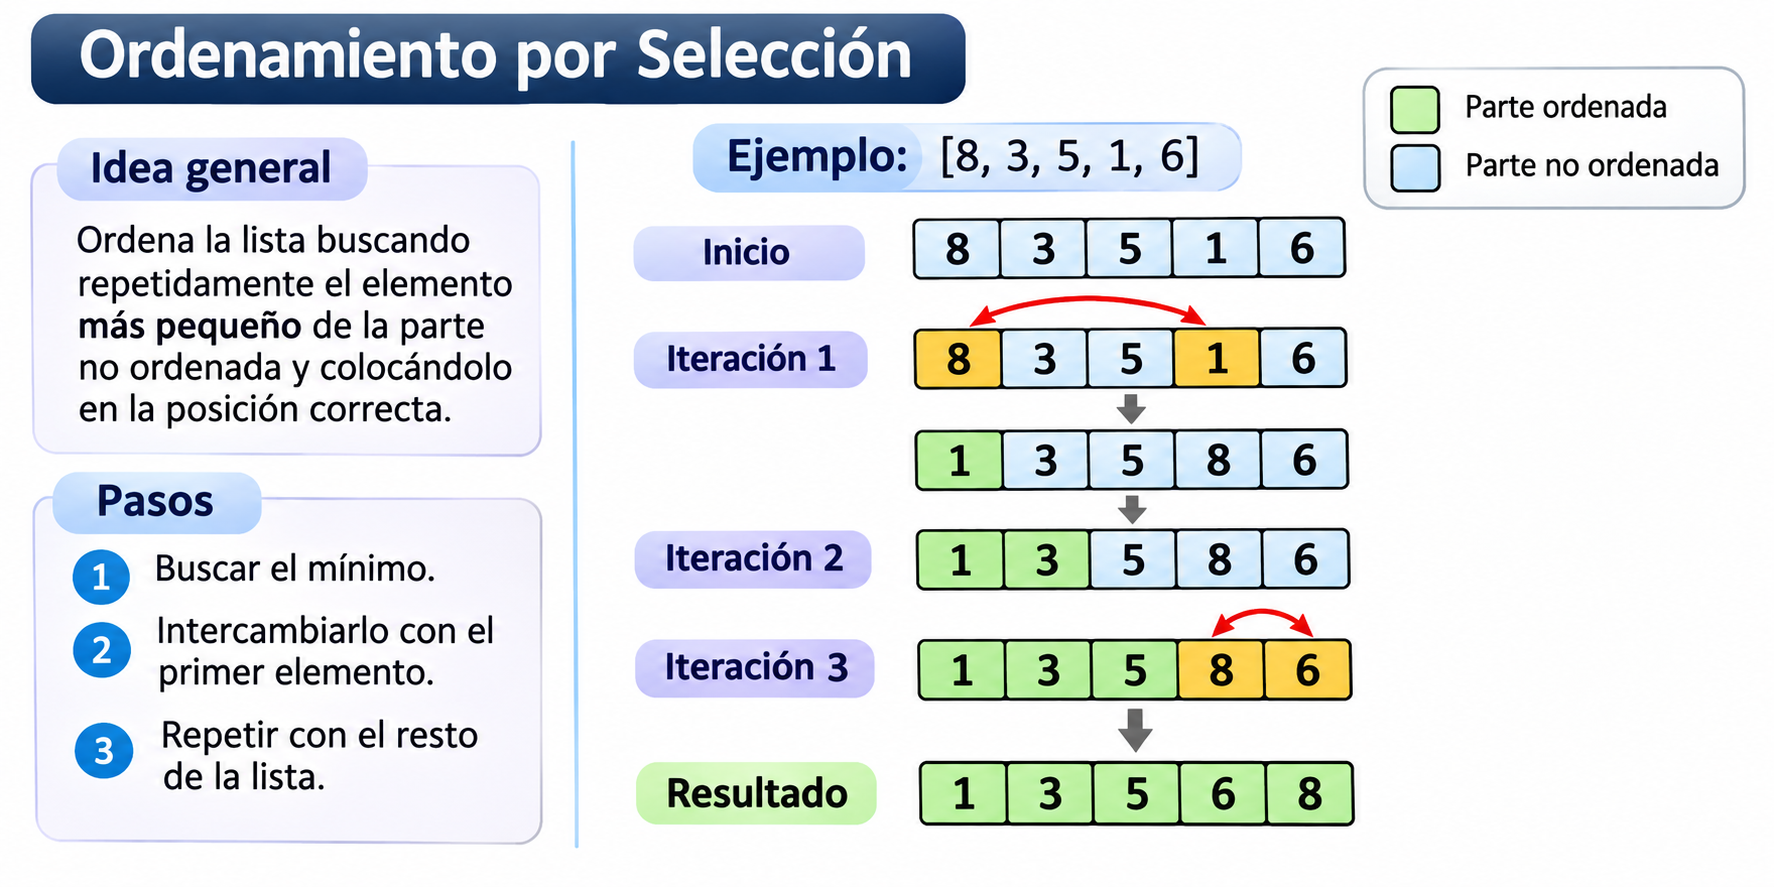
\includegraphics[width=\textwidth]{SelectionSort.png}
        \end{figure}
    \end{frame}

    \begin{frame}[fragile, t]{Algoritmo de selección: ejemplo manual}
        \begin{minted}[xleftmargin=-2cm, frame=leftline, fontsize=\scriptsize]{python}
            def ordenamiento_seleccion(lista):
                n = len(lista)
                for i in range(n - 1):
                    indice_minimo = i
                    for j in range(i + 1, n):
                        if lista[j] < lista[indice_minimo]:
                            indice_minimo = j
                    lista[i], lista[indice_minimo] = (
                        lista[indice_minimo],
                        lista[i]
                    )

            numeros = [8, 3, 5, 1, 6]
            ordenamiento_seleccion(numeros)
            print(numeros)
            # [1, 3, 5, 6, 8]
        \end{minted}
    \end{frame}

    \begin{frame}{Eficiencia de los algoritmos de ordenamiento}
        Los algoritmos difieren en:
        \begin{itemize}
            \item Complejidad temporal: número de comparaciones y movimientos.
            \item Complejidad espacial: memoria adicional requerida.
        \end{itemize}
        La cantidad de comparaciones para el algoritmo de selección es: \textbf{$\frac{n(n-1)}{2}$}.
        Significa que cuando $n$ es grande, el algoritmo de selección es muy ineficiente.

        \vspace{0.5em}
        \renewcommand{\arraystretch}{1.3}
        \begin{center}
            \footnotesize
            \begin{tabular}{@{}r r@{}}
                \toprule
                \textbf{Elementos} & \textbf{Comparaciones} \\
                \midrule
                5 & 10 \\
                10 & 45 \\
                100 & 4.950 \\
                1.000 & 499.500 \\
                \bottomrule
            \end{tabular}
        \end{center}
    \end{frame}

    %------------------------------------------------------------------

    \begin{frame}[fragile, t]{Ejercicio 1: Completar}
        Complete los espacios en blanco.
        \begin{minted}[xleftmargin=-2cm, frame=leftline, fontsize=\small]{python}
            precios = [4500, 1200, 3890, 990]
            precios.________()
            print(precios)  # creciente

            precios.________(________=True)
            print(precios)  # decreciente

            nombres = ["Zoe", "Ana", "Luis", "Bea"]
            nombres.sort(key=________)
            print(nombres)  # por longitud
        \end{minted}
    \end{frame}

    \begin{frame}[fragile, t]{Ejercicio 1: Solución}
        \begin{minted}[xleftmargin=-2cm, frame=leftline, fontsize=\small]{python}
            precios = [4500, 1200, 3890, 990]
            precios.sort()
            print(precios)  # [990, 1200, 3890, 4500]

            precios.sort(reverse=True)
            print(precios)  # [4500, 3890, 1200, 990]

            nombres = ["Zoe", "Ana", "Luis", "Bea"]
            nombres.sort(key=len)
            print(nombres)  # ['Zoe', 'Ana', 'Bea', 'Luis']
        \end{minted}
    \end{frame}

    \begin{frame}[fragile, t]{Ejercicio 2: Notas por promedio}
        Se tiene una lista de listas \texttt{[nombre, nota]}.
        Ordene de mayor a menor nota. En empate, ordene por nombre.
        \begin{minted}[xleftmargin=-2cm, frame=leftline, fontsize=\scriptsize]{python}
            registro = [
                ["Valentina", 5.5],
                ["Tomás", 6.0],
                ["Antonia", 5.5],
                ["Ignacio", 4.0]
            ]

            def criterio(fila):
                # Completar: varios criterios (piense en el signo para
                # lograr orden decreciente en la nota)
                return ________

            registro.sort(key=criterio)
            print(registro)
        \end{minted}
    \end{frame}

    \begin{frame}[fragile, t]{Ejercicio 2: Solución}
        Una forma es usar el negativo de la nota como primer criterio:
        \begin{minted}[xleftmargin=-2cm, frame=leftline, fontsize=\scriptsize]{python}
            def criterio(fila):
                return (-fila[1], fila[0])

            registro.sort(key=criterio)
            print(registro)
            # [['Tomás', 6.0], ['Antonia', 5.5],
            #  ['Valentina', 5.5], ['Ignacio', 4.0]]
        \end{minted}
    \end{frame}

    %------------------------------------------------------------------
    \begin{frame}{Resumen}
        \begin{itemize}
            \item \mintinline{python}{lista.sort()} ordena de forma creciente y modifica la lista.
            \pause
            \item \mintinline{python}{sort(reverse=True)} ordena en forma decreciente.
            \pause
            \item \mintinline{python}{sort(key=...)} permite un criterio propio
            (atributo, columna, longitud, etc.).
            \pause
            \item Varios criterios se combinan en una tupla: valores separados por comas.
            \pause
            \item El algoritmo de selección ilustra cómo ordenar con comparaciones
            e intercambios.
            \pause
            \item Existen algoritmos más eficientes; en la práctica, Python ya ofrece
            \mintinline{python}{sort()} como herramienta conveniente.
        \end{itemize}
    \end{frame}

\end{document}
